\chapter{序列检测器——状态机的核心应用}

\section{什么是序列检测器}

\textbf{序列检测器}：在串行输入流中检测特定模式的电路。

输入：一串bit流（每个时钟周期输入1bit）
输出：当检测到目标序列时，输出=1

\begin{keypoint}[序列检测器的本质]
序列检测器\textbf{一定}是一个状态机。

为什么？因为它需要"记住已经匹配了序列的前几位"——
这需要\textbf{记忆}。组合逻辑做不到——它不记得历史。
\end{keypoint}

\section{为什么序列检测器一定是状态机}

考虑检测序列1011：

假设当前输入流是：... 1 0 1 ...

此时你看到了"101"，还剩一个"1"就匹配成功。

这个"已经匹配了3位"的信息必须被记住。下一拍如果输入是1，就检测到了；如果是0，就需要重新开始匹配。

\textbf{这个"记住了多少"就是状态。}

\begin{keypoint}[状态在序列检测器中的含义]
状态 = "目前已匹配了目标序列的前几位"

\begin{itemize}
  \item S0（初始）：匹配了0位（等待序列开始）
  \item S1：匹配了1位
  \item S2：匹配了2位
  \item S3：匹配了3位
  \item S4（检测到）：匹配了4位（完整序列！）
\end{itemize}
\end{keypoint}

\section{1011序列检测器——Moore型（可重叠检测）}

\subsection{状态定义（5状态严格Moore）}

检测目标：1011。Moore型使用\textbf{5个状态}，S4为专用输出状态。

\begin{center}
\begin{tabular}{|c|l|c|}
\hline
\textbf{状态} & \textbf{含义（已匹配的前缀）} & \textbf{输出 y} \\
\hline
S0 & 初始状态，未匹配任何位 & 0 \\
S1 & 匹配第1位 "1" & 0 \\
S2 & 匹配前2位 "10" & 0 \\
S3 & 匹配前3位 "101" & 0 \\
S4 & 匹配完整序列 "1011" & \textbf{1} \\
\hline
\end{tabular}
\end{center}

\subsection{状态转移图}

\begin{center}
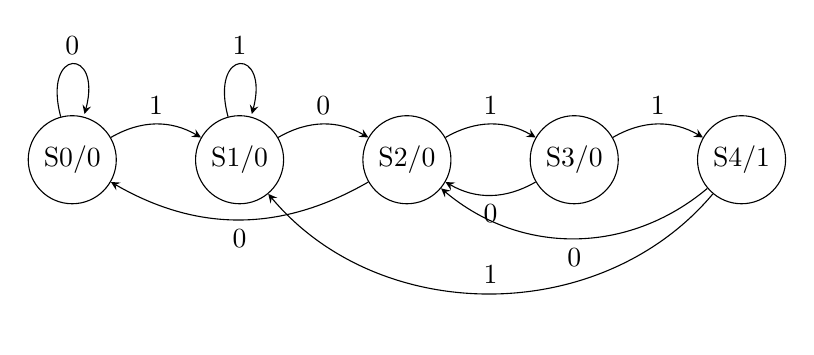
\begin{tikzpicture}[->, >=stealth, node distance=3cm, auto, scale=0.85]
  \node[draw, circle] (S0) at (0,0) {S0/0};
  \node[draw, circle] (S1) at (2.5,0) {S1/0};
  \node[draw, circle] (S2) at (5,0) {S2/0};
  \node[draw, circle] (S3) at (7.5,0) {S3/0};
  \node[draw, circle] (S4) at (10,0) {S4/1};

  \draw (S0) edge[loop above] node{0} (S0);
  \draw (S0) edge[bend left] node{1} (S1);
  \draw (S1) edge[loop above] node{1} (S1);
  \draw (S1) edge[bend left] node{0} (S2);
  \draw (S2) edge[bend left] node{0} (S0);
  \draw (S2) edge[bend left] node{1} (S3);
  \draw (S3) edge[bend left] node{0} (S2);
  \draw (S3) edge[bend left] node{1} (S4);
  \draw (S4) edge[bend left=40] node{0} (S2);
  \draw (S4) edge[bend left=50] node[above]{1} (S1);
\end{tikzpicture}
\end{center}

\textbf{Moore型标注规则：}输出标在状态圈内（状态名/输出值），转移弧上只标输入值。S0-S3输出为0，S4输出为1。

\subsection{状态转移分析}

\begin{itemize}
  \item \textbf{S0}：din=0→S0；din=1→S1
  \item \textbf{S1}：din=0→S2；din=1→S1（"11"的后一个1仍是有效前缀）
  \item \textbf{S2}：din=0→S0；din=1→S3
  \item \textbf{S3}：din=0→S2（"1010"的后缀"10"匹配前缀）；din=1→S4
  \item \textbf{S4}：din=0→S2；din=1→S1（\textbf{可重叠}：末尾1可作为下一组序列起始）
\end{itemize}

\subsection{状态转移表}

\begin{center}
\begin{tabular}{|c|c|c||c|}
\hline
\textbf{当前状态} & \textbf{输入 din} & \textbf{下一状态} & \textbf{输出 y} \\
\hline
S0 & 0 & S0 & 0 \\
S0 & 1 & S1 & 0 \\
S1 & 0 & S2 & 0 \\
S1 & 1 & S1 & 0 \\
S2 & 0 & S0 & 0 \\
S2 & 1 & S3 & 0 \\
S3 & 0 & S2 & 0 \\
S3 & 1 & S4 & 0 \\
S4 & 0 & S2 & 1 \\
S4 & 1 & S1 & 1 \\
\hline
\end{tabular}
\end{center}

\subsection{VHDL实现（两段式，异步高电平复位）}

\begin{lstlisting}[caption={Moore型1011序列检测器（5状态，可重叠）}]
library ieee;
use ieee.std_logic_1164.all;

entity seq1011_moore is
  port(
    clk : in  std_logic;   -- 系统时钟，上升沿有效
    rst : in  std_logic;   -- 异步高电平复位
    din : in  std_logic;   -- 串行数据输入
    y   : out std_logic    -- 检测输出，高电平表示检测到1011
  );
end entity seq1011_moore;

architecture behav of seq1011_moore is
  type state_type is (S0, S1, S2, S3, S4);
  signal curr_state, next_state : state_type;
begin
  -- 第一段：时序逻辑（状态寄存器，时钟+异步复位）
  reg_proc: process(clk, rst)
  begin
    if rst = '1' then
      curr_state <= S0;
    elsif rising_edge(clk) then
      curr_state <= next_state;
    end if;
  end process reg_proc;

  -- 第二段：组合逻辑（状态转移判断）
  comb_proc: process(curr_state, din)
  begin
    case curr_state is
      when S0 =>
        if din = '1' then next_state <= S1;
        else next_state <= S0; end if;
      when S1 =>
        if din = '0' then next_state <= S2;
        else next_state <= S1; end if;
      when S2 =>
        if din = '1' then next_state <= S3;
        else next_state <= S0; end if;
      when S3 =>
        if din = '1' then next_state <= S4;
        else next_state <= S2; end if;
      when S4 =>
        if din = '1' then next_state <= S1;   -- 重叠
        else next_state <= S2; end if;
      when others =>
        next_state <= S0;
    end case;
  end process comb_proc;

  -- Moore型输出：仅由当前状态决定
  y <= '1' when curr_state = S4 else '0';
end architecture behav;
\end{lstlisting}

\section{1101序列检测器（Moore型）}

检测目标：1101。5状态严格Moore，S4为专用输出状态。

状态定义：
\begin{itemize}
  \item S0：初始（匹配0位）\quad S1：已匹配"1"\quad S2：已匹配"11"
  \item S3：已匹配"110"\quad S4：匹配完整序列"1101"，输出y=1
\end{itemize}

\begin{center}
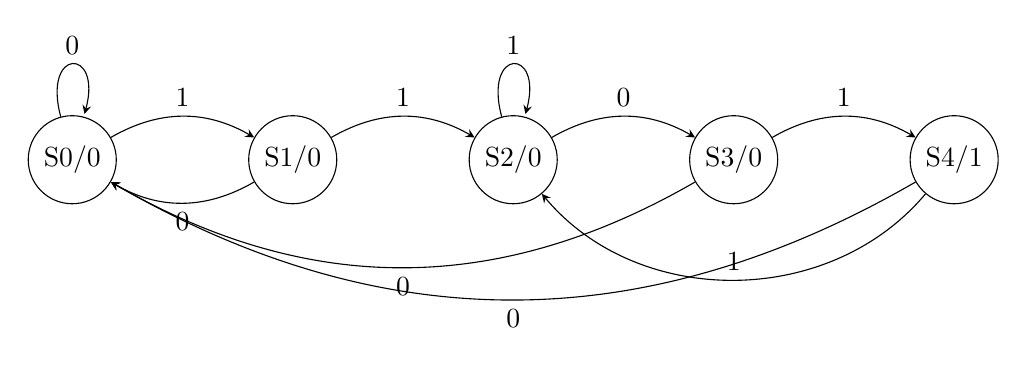
\begin{tikzpicture}[->, >=stealth, node distance=2.8cm, auto]
  \node[draw, circle] (S0) at (0,0) {S0/0};
  \node[draw, circle] (S1) at (2.8,0) {S1/0};
  \node[draw, circle] (S2) at (5.6,0) {S2/0};
  \node[draw, circle] (S3) at (8.4,0) {S3/0};
  \node[draw, circle] (S4) at (11.2,0) {S4/1};

  \draw (S0) edge[loop above] node{0} (S0);
  \draw (S0) edge[bend left] node{1} (S1);
  \draw (S1) edge[bend left] node{0} (S0);
  \draw (S1) edge[bend left] node{1} (S2);
  \draw (S2) edge[loop above] node{1} (S2);
  \draw (S2) edge[bend left] node{0} (S3);
  \draw (S3) edge[bend left] node{0} (S0);
  \draw (S3) edge[bend left] node{1} (S4);
  \draw (S4) edge[bend left=30] node{0} (S0);
  \draw (S4) edge[bend left=50] node[above]{1} (S2);
\end{tikzpicture}
\end{center}

状态转移：S0+1→S1, S1+1→S2, S2+0→S3, S3+1→S4（检测到！）。S4+0→S0, S4+1→S2（重叠：末尾的"1"可开始新序列）。

\section{重叠检测 vs 非重叠检测}

这是\textbf{必考的区别}！

\begin{definition}[重叠检测]
检测到序列后，已匹配的后缀可以用于下一次匹配。

例：输入 ...1011011...（检测1011，重叠）

第一次检测：1 0 \textbf{1 1} 0 1 1 → 在位置4检测到1011
第二次检测：1 0 1 \textbf{1 0 1 1} → 位置4的"11"中的第二个"1"开始新匹配
\end{definition}

\begin{definition}[非重叠检测]
检测到序列后，重新从初始状态开始。

例：输入 ...1011011...（检测1011，非重叠）

第一次检测：1 0 \textbf{1 1} 0 1 1 → 在位置4检测到1011
第二次检测：1 0 1 1 \textbf{0 1 1} ... → 从位置5重新开始（忽略位置4的后缀）
\end{definition}

\textbf{写作VHDL的区别}：

重叠检测：在检测到状态，根据输入决定返回哪个状态（可能有重叠前缀）
非重叠检测：检测到后，直接回到S0/S1（看具体情况）

\section{Moore型 vs Mealy型——考试必考核心对比}

\subsection{两种状态机模型的根本区别}

\begin{keypoint}[Moore vs Mealy的本质]
\textbf{Moore型状态机}：输出\textbf{仅取决于当前状态}。

\textbf{Mealy型状态机}：输出取决于\textbf{当前状态 + 当前输入}。

这个区别看似微小，但导致了两者在\textbf{状态数}、\textbf{输出时序}和\textbf{硬件结构}上的显著差异。
\end{keypoint}

\subsection{Moore型1011序列检测器（5状态）}

\textbf{【状态定义】}严格Moore型使用5个状态，S4为专用输出状态。

\begin{center}
\begin{tabular}{|c|l|c|}\hline
状态 & 含义 & 输出 y \\ \hline
S0 & 未匹配任何有效前缀（初始/复位）& 0 \\
S1 & 已匹配第1位："1" & 0 \\
S2 & 已匹配前2位："10" & 0 \\
S3 & 已匹配前3位："101" & 0 \\
S4 & 匹配完整序列"1011" & \textbf{1} \\ \hline
\end{tabular}
\end{center}

\textbf{【状态转移图】}输出标在状态圈内（Moore型标志）。

\begin{center}
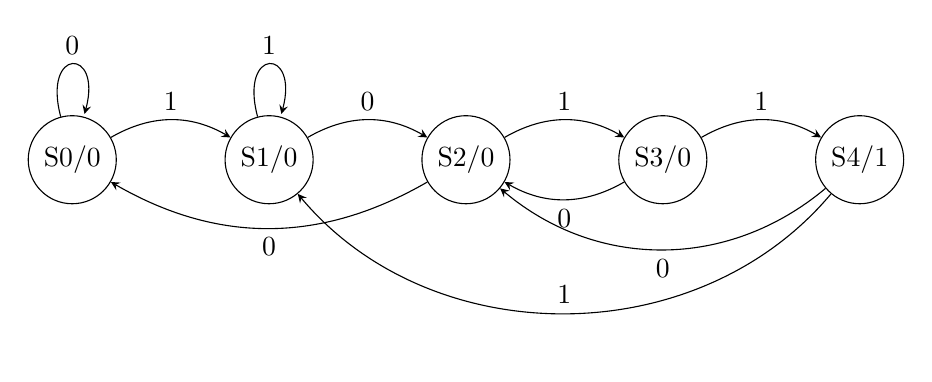
\begin{tikzpicture}[->,>=stealth,node distance=2.5cm,auto]
\node[draw,circle] (S0) at (0,0) {S0/0};
\node[draw,circle] (S1) at (2.5,0) {S1/0};
\node[draw,circle] (S2) at (5,0) {S2/0};
\node[draw,circle] (S3) at (7.5,0) {S3/0};
\node[draw,circle] (S4) at (10,0) {S4/1};
\draw (S0) edge[loop above] node{0} (S0);
\draw (S0) edge[bend left] node{1} (S1);
\draw (S1) edge[loop above] node{1} (S1);
\draw (S1) edge[bend left] node{0} (S2);
\draw (S2) edge[bend left] node{0} (S0);
\draw (S2) edge[bend left] node{1} (S3);
\draw (S3) edge[bend left] node{0} (S2);
\draw (S3) edge[bend left] node{1} (S4);
\draw (S4) edge[bend left=40] node{0} (S2);
\draw (S4) edge[bend left=50] node[above]{1} (S1);
\end{tikzpicture}
\end{center}

\textbf{【输出逻辑】}严格Moore型，$y=1$ 当且仅当 $curr\_state=S4$，与当前输入din无关。进入S4后输出持续整个状态周期（稳定无毛刺）。

\subsection{Mealy型1011序列检测器（4状态）}

\textbf{【状态定义】}Mealy型用4个状态，无专用输出状态，输出在转移弧上。

\begin{center}
\begin{tabular}{|c|l|}\hline
状态 & 含义 \\ \hline
S0 & 未匹配任何有效前缀 \\
S1 & 已匹配第1位："1" \\
S2 & 已匹配前2位："10" \\
S3 & 已匹配前3位："101" \\ \hline
\end{tabular}
\end{center}

\textbf{【状态转移图（标注格式：输入/输出）】}

\begin{center}
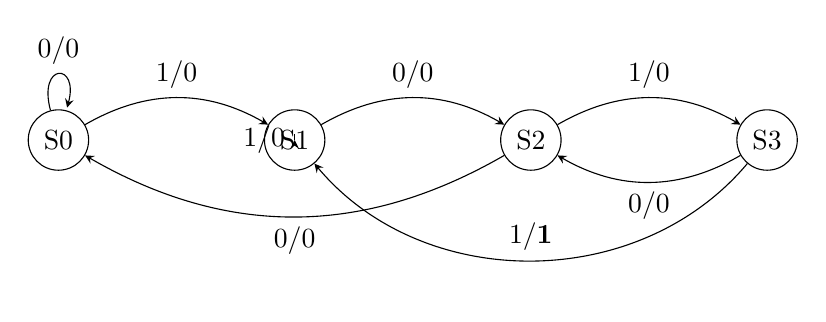
\begin{tikzpicture}[->,>=stealth,node distance=3cm,auto]
\node[draw,circle] (S0) at (0,0) {S0};
\node[draw,circle] (S1) at (3,0) {S1};
\node[draw,circle] (S2) at (6,0) {S2};
\node[draw,circle] (S3) at (9,0) {S3};
\draw (S0) edge[loop above] node{0/0} (S0);
\draw (S0) edge[bend left] node{1/0} (S1);
\draw (S1) edge[bend left] node{1/0} (S1);
\draw (S1) edge[bend left] node{0/0} (S2);
\draw (S2) edge[bend left] node{0/0} (S0);
\draw (S2) edge[bend left] node{1/0} (S3);
\draw (S3) edge[bend left=30] node{0/0} (S2);
\draw (S3) edge[bend left=50] node[above]{1/\textbf{1}} (S1);
\end{tikzpicture}
\end{center}

$S3 \xrightarrow{1/1} S1$：输入=1时y=1（检测到1011），去S1（可重叠——末尾1作新序列起始）。

\textbf{【关键对比】}
\begin{itemize}
  \item \textbf{Moore：5状态(S0-S4)}，输出仅取决于当前状态，$y=1$ when $curr\_state=S4$
  \item \textbf{Mealy：4状态(S0-S3)}，无S4，输出在S3+din=1的转移弧上直接产生
  \item Moore输出晚1拍（等状态稳定），Mealy输出与输入同步
\end{itemize}

\subsection{完整对比表}

\begin{center}
\begin{tabular}{|l|c|c|}\hline
\textbf{对比维度} & \textbf{Moore型} & \textbf{Mealy型} \\ \hline
输出决定因素 & 仅当前状态 & 状态 + 输入 \\ \hline
状态数(检测1011) & 5个(S0-S4) & 4个(S0-S3) \\ \hline
输出时序 & 进入S4后输出（晚1拍）& 转移同时输出（同步）\\ \hline
输出持续时间 & 整个S4周期（稳定）& 仅在条件满足时 \\ \hline
对输入毛刺敏感 & 不敏感（只看状态）& 敏感（输入参与输出）\\ \hline
状态图标注 & 状态圈内"状态/输出"& 转移弧上"输入/输出"\\ \hline
综合结果 & 3FF+输出逻辑 & 2FF+次态/输出组合逻辑 \\ \hline
考试推荐 & 更安全稳定，优先使用 & 更紧凑，按题目要求 \\ \hline
\end{tabular}
\end{center}

\subsection{VHDL实现对比（两段式，异步高电平复位）}

\textbf{【Moore型——5状态，可重叠】}

\begin{lstlisting}[caption={Moore型1011序列检测器}]
library ieee;
use ieee.std_logic_1164.all;

entity seq1011_moore is
  port(
    clk : in  std_logic;
    rst : in  std_logic;   -- 异步高电平复位
    din : in  std_logic;
    y   : out std_logic
  );
end entity seq1011_moore;

architecture behav of seq1011_moore is
  type state_type is (S0, S1, S2, S3, S4);
  signal curr_state, next_state : state_type;
begin
  -- 第一段：时序逻辑（状态寄存器）
  reg_proc: process(clk, rst)
  begin
    if rst = '1' then curr_state <= S0;
    elsif rising_edge(clk) then curr_state <= next_state;
    end if;
  end process reg_proc;

  -- 第二段：组合逻辑（状态转移）
  comb_proc: process(curr_state, din)
  begin
    case curr_state is
      when S0 =>
        if din = '1' then next_state <= S1;
        else next_state <= S0; end if;
      when S1 =>
        if din = '0' then next_state <= S2;
        else next_state <= S1; end if;
      when S2 =>
        if din = '1' then next_state <= S3;
        else next_state <= S0; end if;
      when S3 =>
        if din = '1' then next_state <= S4;
        else next_state <= S2; end if;
      when S4 =>
        if din = '1' then next_state <= S1;   -- 重叠
        else next_state <= S2; end if;
      when others => next_state <= S0;
    end case;
  end process comb_proc;

  -- Moore输出：仅由当前状态决定
  y <= '1' when curr_state = S4 else '0';
end architecture behav;
\end{lstlisting}

\textbf{【Mealy型——4状态，可重叠，默认赋值】}

\begin{lstlisting}[caption={Mealy型1011序列检测器}]
library ieee;
use ieee.std_logic_1164.all;

entity seq1011_mealy is
  port(
    clk : in  std_logic;
    rst : in  std_logic;   -- 异步高电平复位
    din : in  std_logic;
    y   : out std_logic
  );
end entity seq1011_mealy;

architecture behav of seq1011_mealy is
  type state_type is (S0, S1, S2, S3);
  signal curr_state, next_state : state_type;
begin
  -- 第一段：时序逻辑（状态寄存器）
  reg_proc: process(clk, rst)
  begin
    if rst = '1' then curr_state <= S0;
    elsif rising_edge(clk) then curr_state <= next_state;
    end if;
  end process reg_proc;

  -- 第二段：组合逻辑（状态转移 + Mealy输出）
  comb_proc: process(curr_state, din)
  begin
    -- 默认赋值，避免组合逻辑锁存
    next_state <= S0;
    y <= '0';

    case curr_state is
      when S0 =>
        if din = '1' then next_state <= S1;
        else next_state <= S0; end if;
      when S1 =>
        if din = '0' then next_state <= S2;
        else next_state <= S1; end if;
      when S2 =>
        if din = '1' then next_state <= S3;
        else next_state <= S0; end if;
      when S3 =>
        if din = '1' then
          next_state <= S1;
          y <= '1';  -- 检测到1011，输出有效（重叠）
        else
          next_state <= S2;
        end if;
      when others => next_state <= S0;
    end case;
  end process comb_proc;
end architecture behav;
\end{lstlisting}

\textbf{【关键代码差异】}
\begin{itemize}
  \item \textbf{Moore}：5状态，输出在进程外：\texttt{y <= '1' when curr\_state = S4 else '0';}
  \item \textbf{Mealy}：4状态，输出在comb\_proc内：\texttt{y <= '1';}（默认为0，检测到时置1）
  \item \textbf{默认赋值}（Mealy必须）：\texttt{next\_state <= S0; y <= '0';} 写在case之前，避免锁存
  \item \textbf{可重叠/非重叠切换}：改S4/S3的din=1跳转——回S0=非重叠，回S1=重叠
\end{itemize}

\subsection{输出时序对比}

\textbf{【Moore型输出晚1拍】}

\begin{center}
\begin{tabular}{|c|c|c|c|c||c|c|}\hline
时钟拍 & 1 & 2 & 3 & 4 & 5 \\ \hline
输入din & 1 & 0 & 1 & 1 & 0 \\ \hline
Moore curr\_state & S1 & S2 & S3 & S4 & S1 \\ \hline
Moore输出y & 0 & 0 & 0 & \textbf{1}（第4拍！）& 0 \\ \hline
\hline
Mealy curr\_state & S1 & S2 & S3 & S1 & S2 \\ \hline
Mealy输出y & 0 & 0 & 0 & \textbf{1}（第4拍！）& 0 \\ \hline
\end{tabular}
\end{center}

注：严格5状态Moore进入S4即输出$y=1$，在第4拍（与Mealy同拍）输出。Moore输出仅取决于当前状态是否为S4，与输入din无关，这是Moore型与Mealy型的根本区别。

\subsection{考试如何选择}

\begin{examtip}[Moore vs Mealy考试策略]
\begin{enumerate}
  \item \textbf{默认选Moore型（5状态）}：状态图更清晰，输出稳定，符合教材规范
  \item \textbf{题目明确要求Mealy型时才用Mealy（4状态）}
  \item \textbf{状态图标注规范}：
  \begin{itemize}
    \item Moore：状态圈内写"状态名/输出值"（如S0/0, S4/1）
    \item Mealy：转移弧上写"输入值/输出值"（如1/1）
  \end{itemize}
  \item \textbf{VHDL必须用两段式}：时序reg\_proc + 组合comb\_proc
  \item \textbf{Mealy必须有默认赋值}：避免组合逻辑锁存
\end{enumerate}
\end{examtip}

\subsection{硬件综合结果对比}

\begin{center}
\begin{tabular}{|l|c|c|}
\hline
\textbf{硬件模块} & \textbf{Moore型} & \textbf{Mealy型} \\
\hline
状态寄存器 & 3个D触发器（编码5状态）& 2个D触发器（编码4状态）\\
次态逻辑 & 组合电路（当前状态+din → 下一状态）& 组合电路（当前状态+din → 下一状态）\\
输出逻辑 & 独立组合电路（仅读当前状态）& 合并于次态逻辑中（读当前状态+din）\\
输出信号y & S4时y=1，与din无关 & S3且din=1时y=1，随转移产生\\
\hline
关键路径延迟 & 寄存器延迟 + 次态逻辑延迟 & 寄存器延迟 + 次态/输出组合延迟 \\
输出毛刺风险 & 低（仅状态变化时输出才变）& 较高（din直接参与输出）\\
\hline
\end{tabular}
\end{center}

\textbf{结论}：Moore型输出稳定、无毛刺，适合对时序要求严格的场合。Mealy型状态少、响应快，但输出可能受输入毛刺影响。考试中优先使用Moore型。

\section{考试常见变式}

\begin{enumerate}
  \item \textbf{变式1：检测1011（重叠）}

  检测后在S3状态，输入1→检测到，同时此1可作为新序列的第一个1，因此去S1（不是S0）。

  \item \textbf{变式2：检测0101}

  状态：S0（初始）→S1（匹配"0"）→S2（匹配"01"）→S3（匹配"010"）。S3+输入1=检测到。

  \item \textbf{变式3：检测1111}

  4个连续的1。状态：S0→S1（1个1）→S2（2个1）→S3（3个1）。S3+输入1=检测到（重叠：保持S3）。

  \item \textbf{变式4：同时检测多个序列}

  如同时检测1011和1101。需要合并两个状态机。

  \item \textbf{变式5：Mealy型 vs Moore型检测器}

  Mealy：输出取决于状态+输入（输出可以早一拍）
  Moore：输出仅取决于状态（输出晚一拍，但更稳定）

  考试通常要求Moore型。
\end{enumerate}

\section{Testbench}

\begin{lstlisting}[caption={Moore型1011序列检测器Testbench（异步高电平复位）}]
library ieee;
use ieee.std_logic_1164.all;

entity seq1011_moore_tb is
end seq1011_moore_tb;

architecture test of seq1011_moore_tb is
  signal clk, rst, din, y : std_logic;
  constant T : time := 20 ns;

  component seq1011_moore is
    port(clk, rst, din : in std_logic; y : out std_logic);
  end component;
begin
  uut: seq1011_moore port map(clk, rst, din, y);

  clk <= not clk after T/2;

  stimulus: process
  begin
    rst <= '1'; wait for 30 ns;  -- 异步高电平复位
    rst <= '0'; wait for 5 ns;

    -- 输入序列：1 0 1 1 0 1 0 1 1（可重叠验证）
    din <= '1'; wait for T;  -- S0→S1
    din <= '0'; wait for T;  -- S1→S2
    din <= '1'; wait for T;  -- S2→S3
    din <= '1'; wait for T;  -- S3→S4, y=1（检测到！）
    din <= '0'; wait for T;
    din <= '1'; wait for T;
    din <= '0'; wait for T;
    din <= '1'; wait for T;
    din <= '1'; wait for T;  -- 第9拍再次检测到！
    wait;
  end process;
end test;
\end{lstlisting}

\begin{examtip}[序列检测器秒杀法]
\textbf{第一步：确定状态}
状态 = 已匹配的序列前缀（每个状态代表匹配了序列的前几位）

\textbf{第二步：画状态图}
对每个状态，考虑输入0和输入1分别去哪里

\textbf{第三步：写状态转移表}

\textbf{第四步：写VHDL}
\begin{itemize}
  \item type定义状态枚举
  \item case语句处理每个状态
  \item 检测到条件：在倒数第二个状态 + 最后一个匹配位
\end{itemize}

\textbf{关键技巧}：状态S3下输入1→检测到。但去哪？
\begin{itemize}
  \item 重叠检测：分析后几位能否作为新前缀→S1（"1011"最后的"1"可以是新序列的第一个"1"）
  \item 非重叠检测：直接回S0
\end{itemize}
\end{examtip}

\section{状态机的其他应用——不止序列检测器}

序列检测器是状态机最经典的应用，但状态机的应用远不止于此。实际上，前面学过的很多电路本质上都是状态机。

\subsection{计数器 = 状态机}

\textbf{用状态机的眼光重新看模6计数器：}

\begin{center}
\begin{tabular}{|c|c|c|}
\hline
\textbf{状态机要素} & \textbf{模6计数器对应} & \textbf{硬件实现} \\
\hline
当前状态 & cnt[2:0]（3位D触发器）& 3个DFF \\
次态逻辑 & $cnt_{next} = cnt + 1$（若$cnt=5$则归0）& 加法器+比较器 \\
输出逻辑 & count = cnt, carry = 1 when cnt=5 & 连线+比较器 \\
\hline
\end{tabular}
\end{center}

\textbf{状态转移图（模6计数器）：}

\begin{center}
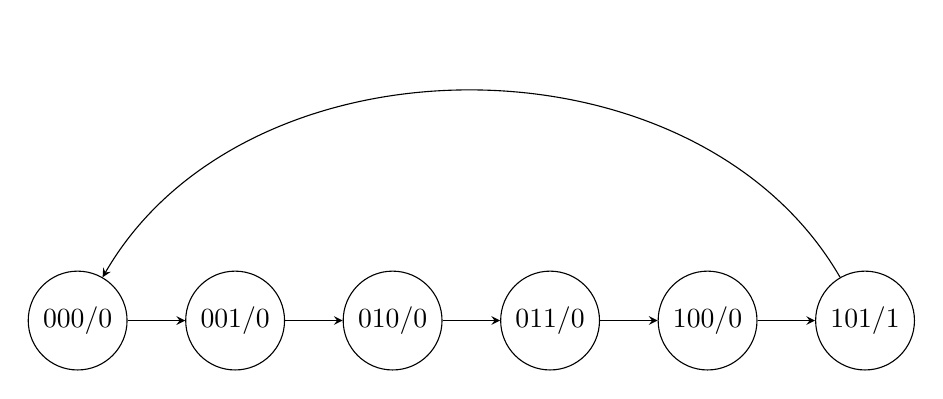
\begin{tikzpicture}[->,>=stealth,node distance=2cm,auto]
\node[draw,circle] (s0) at (0,0) {000/0};
\node[draw,circle] (s1) at (2,0) {001/0};
\node[draw,circle] (s2) at (4,0) {010/0};
\node[draw,circle] (s3) at (6,0) {011/0};
\node[draw,circle] (s4) at (8,0) {100/0};
\node[draw,circle] (s5) at (10,0) {101/1};
\draw (s0) -- (s1); \draw (s1) -- (s2); \draw (s2) -- (s3);
\draw (s3) -- (s4); \draw (s4) -- (s5);
\draw (s5) edge[bend right=60] (s0);
\end{tikzpicture}
\end{center}
（状态标注格式：计数值/carry输出）

\textbf{用直观状态机写法重写模6计数器：}

\begin{lstlisting}[caption={模6计数器——每个状态一行，输出和下一拍一起写}]
architecture Behavioral of counter_mod6_fsm is
  type state is (s0,s1,s2,s3,s4,s5);
  signal present_state, next_state: state;
begin
  process(rst, clk)
  begin
    if rst='0' then present_state <= s0;
    elsif clk'event and clk='1' then
      present_state <= next_state;
    end if;
  end process;

  COM: process(present_state)
  begin
    case present_state is
      when s0 => count<="000"; carry<='0'; next_state<=s1;
      when s1 => count<="001"; carry<='0'; next_state<=s2;
      when s2 => count<="010"; carry<='0'; next_state<=s3;
      when s3 => count<="011"; carry<='0'; next_state<=s4;
      when s4 => count<="100"; carry<='0'; next_state<=s5;
      when s5 => count<="101"; carry<='1'; next_state<=s0;
      when others => count<="000"; carry<='0'; next_state<=s0;
    end case;
  end process COM;
end Behavioral;
\end{lstlisting}

\textbf{对比：}上面用的是\textbf{枚举6个状态}的写法（6个when分支），下面是用加法器+清零的写法：

\begin{lstlisting}[caption={模6计数器——传统写法（等价但更简洁）}]
  if cnt = 5 then cnt <= 0; else cnt <= cnt + 1; end if;
\end{lstlisting}

两段代码\textbf{完全等价}——综合出来的硬件一模一样。但枚举写法让你看清：计数器就是一个6状态的循环状态机。

\textbf{拓展练习：用状态机实现模5计数器}

将上面模6的方法直接套用到模5：5个状态s0-s4。

\begin{lstlisting}[caption={模5计数器——直观状态机写法}]
type state is (s0,s1,s2,s3,s4);
signal present_state, next_state: state;
...
COM: process(present_state)
begin
  case present_state is
    when s0 => count<="000"; next_state<=s1;
    when s1 => count<="001"; next_state<=s2;
    when s2 => count<="010"; next_state<=s3;
    when s3 => count<="011"; next_state<=s4;
    when s4 => count<="100"; next_state<=s0;
    when others => count<="000"; next_state<=s0;
  end case;
end process COM;
\end{lstlisting}

\textbf{任意模N计数器都可以这样写——N个状态，N个when分支。}每个分支写清楚当前状态输出什么值、下一拍去哪里。模12=12行，模24=24行，以此类推。

\subsection{分频器 = 状态机}

分频器的本质：一个状态在$M$个状态间循环，输出在特定状态翻转。

\textbf{例题：12分频器（占空比50\%）。}$M=12$，需要12个状态。前6个状态输出0，后6个状态输出1。

\textbf{状态转移图（12状态循环）：}
\begin{center}
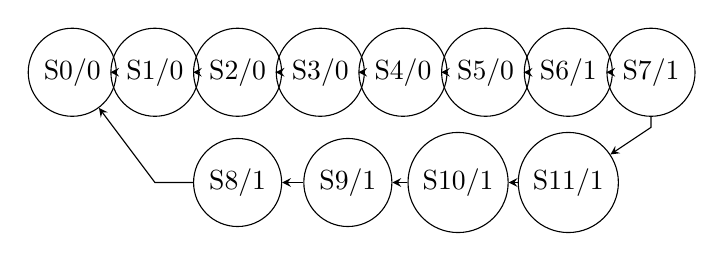
\begin{tikzpicture}[->,>=stealth,node distance=1.3cm,auto,scale=0.7]
\node[draw,circle] (s0) at (0,0) {S0/0};
\node[draw,circle] (s1) at (1.5,0) {S1/0};
\node[draw,circle] (s2) at (3,0) {S2/0};
\node[draw,circle] (s3) at (4.5,0) {S3/0};
\node[draw,circle] (s4) at (6,0) {S4/0};
\node[draw,circle] (s5) at (7.5,0) {S5/0};
\node[draw,circle] (s6) at (9,0) {S6/1};
\node[draw,circle] (s7) at (10.5,0) {S7/1};
\node[draw,circle] (s8) at (3,-2) {S8/1};
\node[draw,circle] (s9) at (5,-2) {S9/1};
\node[draw,circle] (sa) at (7,-2) {S10/1};
\node[draw,circle] (sb) at (9,-2) {S11/1};
\draw (s0)--(s1); \draw (s1)--(s2); \draw (s2)--(s3); \draw (s3)--(s4);
\draw (s4)--(s5); \draw (s5)--(s6); \draw (s6)--(s7);
\draw (s7) -- (10.5,-1) -- (sb);
\draw (sb)--(sa); \draw (sa)--(s9); \draw (s9)--(s8);
\draw (s8) -- (1.5,-2) -- (s0);
\end{tikzpicture}
\end{center}
（S0-S5输出0，S6-S11输出1，12个状态循环。6拍低+6拍高=50\%占空比。）

\textbf{VHDL——直观状态机写法：}
\begin{lstlisting}[caption={12分频器——每个状态一行，输出和转移一起写}]
architecture Behavioral of div12_fsm is
  type state is (s0,s1,s2,s3,s4,s5,s6,s7,s8,s9,s10,s11);
  signal present_state, next_state: state;
begin
  process(rst, clk)
  begin
    if rst='0' then present_state <= s0;
    elsif clk'event and clk='1' then
      present_state <= next_state;
    end if;
  end process;

  COM: process(present_state)
  begin
    case present_state is
      when s0  => clk_out<='0'; next_state<=s1;
      when s1  => clk_out<='0'; next_state<=s2;
      when s2  => clk_out<='0'; next_state<=s3;
      when s3  => clk_out<='0'; next_state<=s4;
      when s4  => clk_out<='0'; next_state<=s5;
      when s5  => clk_out<='0'; next_state<=s6;
      when s6  => clk_out<='1'; next_state<=s7;
      when s7  => clk_out<='1'; next_state<=s8;
      when s8  => clk_out<='1'; next_state<=s9;
      when s9  => clk_out<='1'; next_state<=s10;
      when s10 => clk_out<='1'; next_state<=s11;
      when s11 => clk_out<='1'; next_state<=s0;
      when others => clk_out<='0'; next_state<=s0;
    end case;
  end process COM;
end Behavioral;
\end{lstlisting}

\textbf{和传统计数器写法对比：}
\begin{lstlisting}[caption={传统写法（模12计数器+比较）}]
if cnt=11 then cnt<=0; else cnt<=cnt+1; end if;
clk_out <= '0' when cnt < 6 else '1';
\end{lstlisting}

同样等价！状态机12状态枚举写法更直观——你看状态图就知道输出波形是什么。计数器写法更紧凑——4位计数器+比较器搞定。\textbf{考试中两种写法都正确，状态机写法更容易画状态转移图拿步骤分。}

\subsection{移位寄存器 = 状态机}

移位寄存器的"状态"就是N个D触发器的内容——一个N位向量，总共$2^N$种可能。次态函数非常简单：$Q_{next} = \{si, Q[N-1:1]\}$（右移）或$\{Q[N-2:0], si\}$（左移）。

\textbf{本质上它是状态机，但次态逻辑太简单了——一行拼接就表达完毕，不需要case枚举。}

\textbf{移位寄存器是状态机——但你不会用case去写它。}

4位移位寄存器有$2^4=16$个状态。\textbf{理论上}可以枚举16个状态用case写——比如状态"0000"输入1→下一拍"1000"；状态"1000"输入0→下一拍"0100"...以此类推，16个状态×2种输入=32个when分支。

\textbf{但没人会这样写}——太蠢了。一行\texttt{reg <= si \& reg(3 downto 1)}就搞定的事情，写32行case毫无意义。

\textbf{这说明一个重要区别：}
\begin{itemize}
  \item 有些电路的次态逻辑\textbf{有简洁的数学表达}（移位=拼接、计数=+1）→ 不需要枚举状态
  \item 有些电路没有（序列检测的前缀匹配、售货机的金额累计）→ \textbf{必须}枚举状态
\end{itemize}

\textbf{什么时候必须用显式状态机？}次态逻辑没有简洁公式时。序列检测器检测1011——你没法用一个数学表达式描述"已匹配101时输入1→检测到"，所以必须枚举S0/S1/S2/S3四个状态。计数器和移位寄存器的次态有简洁公式（+1和拼接），用传统写法即可。

\textbf{环形计数器和Johnson计数器}是移位寄存器的特例：反馈线不同，同样不需要显式状态机。

\subsection{序列发生器 = 状态机}

序列发生器是\textbf{无外部输入的状态机}— 没有din，次态只取决于当前状态。以序列00011101为例：

\textbf{状态转移图（8状态，无输入）：}

\begin{center}
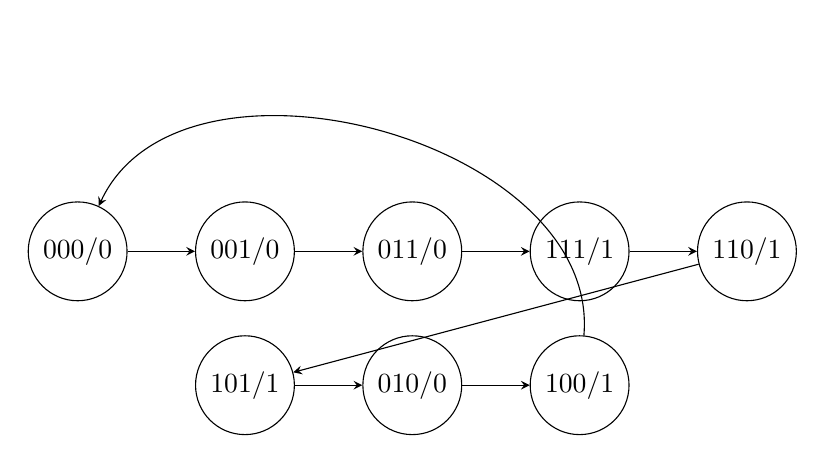
\begin{tikzpicture}[->,>=stealth,node distance=1.8cm,auto,scale=0.85]
\node[draw,circle] (s0) at (0,0) {000/0};
\node[draw,circle] (s1) at (2.5,0) {001/0};
\node[draw,circle] (s2) at (5,0) {011/0};
\node[draw,circle] (s3) at (7.5,0) {111/1};
\node[draw,circle] (s4) at (10,0) {110/1};
\node[draw,circle] (s5) at (2.5,-2) {101/1};
\node[draw,circle] (s6) at (5,-2) {010/0};
\node[draw,circle] (s7) at (7.5,-2) {100/1};
\draw (s0) -- (s1); \draw (s1) -- (s2); \draw (s2) -- (s3);
\draw (s3) -- (s4); \draw (s4) -- (s5); \draw (s5) -- (s6);
\draw (s6) -- (s7); \draw (s7) edge[bend right=80] (s0);
\end{tikzpicture}
\end{center}
（状态标注格式：Q/输出值。转移弧上无标注——因为没有外部输入。）

\textbf{注意和序列检测器的对比：}
\begin{itemize}
  \item 检测器弧上有输入值(0/1)，因为去哪取决于din
  \item 发生器弧上没有输入，因为去哪是确定的（CASE表写死了）
\end{itemize}

\textbf{用状态机写法实现：}

\begin{lstlisting}[caption={序列发生器00011101——直观状态机写法}]
architecture Behavioral of seqgen_fsm is
  type state is (s0,s1,s2,s3,s4,s5,s6,s7);
  signal present_state, next_state: state;
begin
  -- 状态寄存器
  process(rst, clk)
  begin
    if rst='0' then present_state <= s0;
    elsif clk'event and clk='1' then
      present_state <= next_state;
    end if;
  end process;

  -- 次态逻辑 + 输出（每个状态一行：输出什么 + 下一拍去哪）
  COM: process(present_state)
  begin
    case present_state is
      when s0 => q <= '0'; next_state <= s1;
      when s1 => q <= '0'; next_state <= s2;
      when s2 => q <= '0'; next_state <= s3;
      when s3 => q <= '1'; next_state <= s4;
      when s4 => q <= '1'; next_state <= s5;
      when s5 => q <= '1'; next_state <= s6;
      when s6 => q <= '0'; next_state <= s7;
      when s7 => q <= '1'; next_state <= s0;
      when others => q <= '0'; next_state <= s0;
    end case;
  end process COM;
end Behavioral;
\end{lstlisting}

\textbf{这种写法的好处：}每个状态一行——\texttt{when s3 => q <= '1'; next\_state <= s4;} → 状态s3输出1，下一拍去s4。8个状态8行，序列00011101直接写在代码里，一目了然。和状态转移图完全对应——图上每个圈写什么，代码里每个when就写什么。

\textbf{和移位寄存器+CASE表写法对比：}两者功能完全相同。状态机枚举写法更直观（8个状态看得清清楚楚），查表写法更紧凑（不需要枚举状态类型）。

\subsection{统一视角}

\begin{center}
\begin{tikzpicture}[>=stealth]
\node[draw,minimum width=3cm,minimum height=1cm] (reg) at (0,0) {状态寄存器(D触发器)};
\node[draw,minimum width=3cm,minimum height=1.2cm] (nsl) at (5,0) {次态逻辑};
\node[draw,minimum width=3cm,minimum height=1cm] (ol) at (5,-2) {输出逻辑};
\draw[->] (reg) -- (nsl) node[midway,above]{当前状态};
\draw[->] (nsl.east) -- ++(1,0) |- (reg.north) node[near end,right]{下一状态};
\draw[->] (reg.east) -- ++(0.5,0) |- (ol.west);
\draw[->] (ol.east) -- ++(1.5,0) node[right]{输出};
\node at (2.5,-3.5) {所有同步时序电路都遵循这个结构};
\end{tikzpicture}
\end{center}

\begin{center}
\begin{tabular}{|l|c|c|c|}
\hline
\textbf{电路} & \textbf{次态逻辑} & \textbf{输出逻辑} & \textbf{输入} \\
\hline
计数器 & $+1$ 加法器 & 计数值/进位 & 无（或en/load）\\
移位寄存器 & 移位拼接 & 并行/串行数据 & si/din \\
序列发生器 & CASE查表 & Q最高位 & 无 \\
序列检测器 & 前缀匹配判断 & detected信号 & din串行输入 \\
\hline
\end{tabular}
\end{center}

\textbf{核心结论：}

\begin{center}
\begin{tabular}{|l|c|c|}
\hline
\textbf{电路} & \textbf{次态逻辑} & \textbf{需要显式状态机？} \\
\hline
计数器 & $cnt+1$（有简洁数学公式）& 不需要，一行cnt<=cnt+1即可 \\
移位寄存器 & 拼接运算（有简洁公式）& 不需要，一行reg<=si\&reg即可 \\
序列发生器 & CASE查表/枚举 & 可以（枚举更直观）\\
序列检测器 & 前缀匹配判断 & \textbf{必须}——没有简洁公式 \\
\hline
\end{tabular}
\end{center}

\textbf{什么时候用显式状态机：次态逻辑没有简洁数学表达式的时候。}计数器+1、移位拼接——一行代码搞定。序列检测的前缀匹配、售货机的金额累计——必须老老实实画状态图、写case枚举。\textbf{不是所有电路都要写成状态机，但所有电路都可以用状态机来理解。}

\section{变式详解}
\chapter{序列检测器——全部变式详解}

\section{变式1：检测1011（重叠 vs 非重叠）}

\begin{detailbox}[完整教学]
\textbf{【核心区别】}S3+输入1→检测到！
\begin{itemize}
  \item \textbf{非重叠}→回S0（重新开始）
  \item \textbf{重叠}→去S1（最后的"1"作为新序列的第一个"1"）
\end{itemize}

\textbf{【重叠检测版本——完整VHDL（Moore型，5状态）】}
\begin{lstlisting}[caption={1011序列检测器——Moore型可重叠}]
library ieee;
use ieee.std_logic_1164.all;

entity seq1011_moore is
  port(
    clk : in  std_logic;
    rst : in  std_logic;   -- 异步高电平复位
    din : in  std_logic;
    y   : out std_logic
  );
end entity seq1011_moore;

architecture behav of seq1011_moore is
  type state_type is (S0, S1, S2, S3, S4);
  signal curr_state, next_state : state_type;
begin
  reg_proc: process(clk, rst)
  begin
    if rst = '1' then curr_state <= S0;
    elsif rising_edge(clk) then curr_state <= next_state;
    end if;
  end process reg_proc;

  comb_proc: process(curr_state, din)
  begin
    case curr_state is
      when S0 =>
        if din = '1' then next_state <= S1;
        else next_state <= S0; end if;
      when S1 =>
        if din = '0' then next_state <= S2;
        else next_state <= S1; end if;
      when S2 =>
        if din = '1' then next_state <= S3;
        else next_state <= S0; end if;
      when S3 =>
        if din = '1' then next_state <= S4;
        else next_state <= S2; end if;
      when S4 =>
        if din = '1' then next_state <= S1;   -- 重叠！末尾1→新序列起始
        else next_state <= S2; end if;
      when others => next_state <= S0;
    end case;
  end process comb_proc;

  y <= '1' when curr_state = S4 else '0';
end architecture behav;
\end{lstlisting}

\textbf{【考试判断】}看S4状态的din=1跳转目标。S4+1→S0=非重叠，S4+1→S1=可重叠。
\end{detailbox}


\section{变式2：检测1101}

\begin{detailbox}[完整教学]
\textbf{【状态】}S0→S1→S2→S3→(输入1=检测到)
\textbf{【重叠处理】}S3+1→检测到→去S2（"1101"中后两位"11"匹配"11"前缀）
\textbf{【关键】}S2+1→S2（"111"中后两个"11"为有效前缀）。

\begin{lstlisting}[caption={1101序列检测器——Moore型可重叠（5状态）}]
library ieee;
use ieee.std_logic_1164.all;

entity seq1101_moore is
  port(
    clk : in  std_logic;
    rst : in  std_logic;
    din : in  std_logic;
    y   : out std_logic
  );
end entity seq1101_moore;

architecture behav of seq1101_moore is
  type state_type is (S0, S1, S2, S3, S4);
  signal curr_state, next_state : state_type;
begin
  reg_proc: process(clk, rst)
  begin
    if rst = '1' then curr_state <= S0;
    elsif rising_edge(clk) then curr_state <= next_state;
    end if;
  end process reg_proc;

  comb_proc: process(curr_state, din)
  begin
    case curr_state is
      when S0 =>
        if din = '1' then next_state <= S1;
        else next_state <= S0; end if;
      when S1 =>
        if din = '0' then next_state <= S0;
        else next_state <= S2; end if;
      when S2 =>
        if din = '0' then next_state <= S3;
        else next_state <= S2; end if;   -- din=1保持S2
      when S3 =>
        if din = '1' then next_state <= S4;
        else next_state <= S0; end if;
      when S4 =>
        if din = '1' then next_state <= S2;   -- 重叠
        else next_state <= S0; end if;
      when others => next_state <= S0;
    end case;
  end process comb_proc;

  -- Moore输出：仅取决于状态
  y <= '1' when curr_state = S4 else '0';
end architecture behav;
\end{lstlisting}
\end{detailbox}


\section{变式3：检测1111（连续4个1）}

\begin{detailbox}[完整教学]
\textbf{【状态】}S0→S1(1个1)→S2(2个1)→S3(3个1)→(第4个1→检测)
\textbf{【特点】}任意时刻输入0→回S0（连续中断）。
\textbf{【重叠】}S3+1→S3（"1111"后3个"111"为有效前缀）。

\begin{lstlisting}[caption={1111序列检测器——Moore型可重叠（5状态）}]
library ieee;
use ieee.std_logic_1164.all;

entity seq1111_moore is
  port(
    clk : in  std_logic;
    rst : in  std_logic;
    din : in  std_logic;
    y   : out std_logic
  );
end entity seq1111_moore;

architecture behav of seq1111_moore is
  type state_type is (S0, S1, S2, S3, S4);
  signal curr_state, next_state : state_type;
begin
  reg_proc: process(clk, rst)
  begin
    if rst = '1' then curr_state <= S0;
    elsif rising_edge(clk) then curr_state <= next_state;
    end if;
  end process reg_proc;

  comb_proc: process(curr_state, din)
  begin
    case curr_state is
      when S0 =>
        if din = '1' then next_state <= S1;
        else next_state <= S0; end if;
      when S1 =>
        if din = '1' then next_state <= S2;
        else next_state <= S0; end if;
      when S2 =>
        if din = '1' then next_state <= S3;
        else next_state <= S0; end if;
      when S3 =>
        if din = '1' then next_state <= S4;
        else next_state <= S0; end if;
      when S4 =>
        if din = '1' then next_state <= S4;   -- 重叠！保持S4
        else next_state <= S0; end if;
      when others => next_state <= S0;
    end case;
  end process comb_proc;

  y <= '1' when curr_state = S4 else '0';
end architecture behav;
\end{lstlisting}
\end{detailbox}


\section{变式4：检测0101}

\begin{detailbox}[完整教学]
\textbf{【状态】}检测0101（4位序列），状态按S0-S3顺序命名，每个状态含义取决于目标序列：
\begin{itemize}
  \item S0：初始（匹配0位）
  \item S1：已匹配"0"（序列第一位）
  \item S2：已匹配"01"（序列前两位）
  \item S3：已匹配"010"（序列前三位，等待最后一位1）
\end{itemize}
\textbf{【注意】}S3+1→检测到；S3+0→S1（重叠："0100"最后的"0"可作为新序列第一个"0"）。

\begin{lstlisting}[caption={0101序列检测器——Moore型可重叠（5状态）}]
library ieee;
use ieee.std_logic_1164.all;

entity seq0101_moore is
  port(
    clk : in  std_logic;
    rst : in  std_logic;
    din : in  std_logic;
    y   : out std_logic
  );
end entity seq0101_moore;

architecture behav of seq0101_moore is
  type state_type is (S0, S1, S2, S3, S4);
  signal curr_state, next_state : state_type;
begin
  reg_proc: process(clk, rst)
  begin
    if rst = '1' then curr_state <= S0;
    elsif rising_edge(clk) then curr_state <= next_state;
    end if;
  end process reg_proc;

  comb_proc: process(curr_state, din)
  begin
    case curr_state is
      when S0 =>
        if din = '0' then next_state <= S1;
        else next_state <= S0; end if;
      when S1 =>
        if din = '1' then next_state <= S2;   -- "01"
        else next_state <= S1; end if;         -- "00"保持
      when S2 =>
        if din = '0' then next_state <= S3;   -- "010"
        else next_state <= S0; end if;
      when S3 =>
        if din = '1' then next_state <= S4;   -- "0101"
        else next_state <= S1; end if;         -- "0100"→S1
      when S4 =>
        if din = '0' then next_state <= S1;   -- 重叠
        else next_state <= S0; end if;
      when others => next_state <= S0;
    end case;
  end process comb_proc;

  y <= '1' when curr_state = S4 else '0';
end architecture behav;
\end{lstlisting}
\end{detailbox}


\section{变式5：用移位寄存器+比较器替代状态机}

\begin{detailbox}[完整教学]
\textbf{【方案】}移位寄存器存最近N位→与目标序列比较。
\textbf{【完整VHDL】}
\begin{lstlisting}[caption={移位寄存器+比较器实现1011序列检测}]
library ieee;
use ieee.std_logic_1164.all;

entity seq_detector_shift is
  port(
    clk : in  std_logic;
    rst : in  std_logic;
    din : in  std_logic;
    y   : out std_logic
  );
end seq_detector_shift;

architecture behavioral of seq_detector_shift is
  signal reg : std_logic_vector(3 downto 0);
begin
  process(clk, rst)
  begin
    if rst = '1' then
      reg <= (others => '0');
    elsif rising_edge(clk) then
      reg <= din & reg(3 downto 1);
    end if;
  end process;

  y <= '1' when reg = "1011" else '0';
end behavioral;
\end{lstlisting}
\textbf{【优点】}代码极简。不需推导状态转移。
\textbf{【注意】}自动实现重叠检测。
\textbf{【考试适用】}除非题目明确要求"用状态机设计"，否则移位寄存器方案是最佳选择。
\end{detailbox}
